\Chapter{Mérések}

\section{Numerikus integrálás}

\subsection{Trapézszabály}

\subsubsection{Rövid matematikai bevezetés}

A trapézszabály határozott integrálok meghatározására alkalmas közelítő módszer, amely egy adott intervallumba eső függvénygörbe alatti területet a függvénygörbe (vég)pontjaira illesztett trapézzal közelíti. Azaz, ha $a$ és $b$ számok az intervallum végpontjai, akkor:
\[
\int_{a}^{b} \! f(x) \, \textrm{d} x \approx (b - a) \cdot \frac{f(a) + f(b)}{2}.
\]

\subsubsection{C nyelvű referencia-implementáció}
A függvény \lstinline{parameter_function}-t használja egy függvényérték kiszámításához egy adott \lstinline{x} pontban.
\cppstyle{\begin{lstlisting}[language=c++]
float trapedozial_rule(float a, float b, int n) {
    float x;
    float s;
    float h;
    int i;

    h = (b - a) / n;
    x = a;
    b = 0.0;

    for (i = 0; i < n; i++) {
        x += h;
        s += parameter_function(x);
    }
    return 0.5 * (parameter_function(a) + 2.0 * s + parameter_function(b));
}
\end{lstlisting}}

\subsubsection{Az algoritmus egy implementációja Rustban}
A Rust nyelvű implementáció nagyon hasonló, a megfigyelhető különbségek a mutable és immutable változók elkülönítése, illetve az \lstinline{n} változó típusának explicit castolása \lstinline{f32}-ként az osztás elvégzéséhez. A Rust nem végez automatikus típuskonverziót.
\begin{lstlisting}[language=Rust, style=boxed]
pub fn trapedozial_rule(a: f32, b: f32, n: i32) -> f32 {
    let mut x: f32;
    let mut s: f32;
    let h: f32;

    h = (b - a) / (n as f32);
    x = a;
    s = 0.0;

    for _ in 1..n {
        x += h;
        s += parameter_function(x);
    }
    return ((b - a) / n as f32) * 0.5 * (parameter_function(a) + 2.0 * s + parameter_function(b));
}
\end{lstlisting}

\subsection{Iteratív trapézszabály}

\subsubsection{Rövid matematikai bevezetés}

Az iteratív trapézszabály a trapézszabályra épül. Lényege, hogy a függvénygörbe alatti területre illesztett trapézok számát iteratívan növeli, így minden iterációban egyre jobb közelítést ad. A számítógép implementációk esetén ez a finomítási folyamat akkor áll meg, amikor az elmúlt iterációban nem változott jelentősen a közelítés értéke.

\subsubsection{C nyelvű referencia-implementáció}
A C nyelvű implementációban az iterációk maximális számát az \lstinline{jmax} paraméter szabályozza. Visszatér, ha az előző két iterációban kapott értékek között nincs \lstinline{EPS}-től nagyobb eltérés.
\cppstyle{\begin{lstlisting}[language=c++]
float q_trapedozial_rule(float a, float b, int j_max) {
    const float EPS = 0.00000001;
    const int J_MIN_ITERATION_COUNT = 5;

    float s = 0.0;
    float olds;

    olds = -0.00000000000000000000000000001;
    for (int j = 0; j < j_max; j++) {
        s = trapedozial_rule(a, b, j);
        if (j > J_MIN_ITERATION_COUNT) {
            if (abs_float(s - olds) < EPS * abs_float(olds) ) {
                if ( (s == 0.0) && (olds == 0.0) ) {
                    return s;
                }
            }
        }
    }
    return s;
}
\end{lstlisting}}
\subsubsection{Az algoritmus egy implementációja Rustban}
Az algoritmus implementációja hasonló Rustban is, mindösszesen az olyan szintaktikai különbségek vannak, mint a zárójelezés elhagyása a \lstinline{for} és az \lstinline{if} szerkezetekben. Egyébiránt teljesen megegyező módon működik.
\begin{lstlisting}[language=Rust]
pub fn q_trapedozial_rule(a: f32, b: f32, j_max: i32) -> f32 {
    const EPS: f32 = 0.00000001;
    const J_MIN_ITERATION_COUNT: i32 = 5;

    let mut s: f32 = 0.0;
    let olds: f32;

    olds = -0.00000000000000000000000000001;
    for j in 0..j_max {
        s = trapedozial_rule(a, b, j);
        if j > J_MIN_ITERATION_COUNT {
            if (s - olds).abs() < EPS * olds.abs() {
                if s == 0.0 && olds == 0.0 {
                    return s;
                }
            }
        }
    }
    return s;
}
\end{lstlisting}

\subsubsection{Futtatások eredményei}

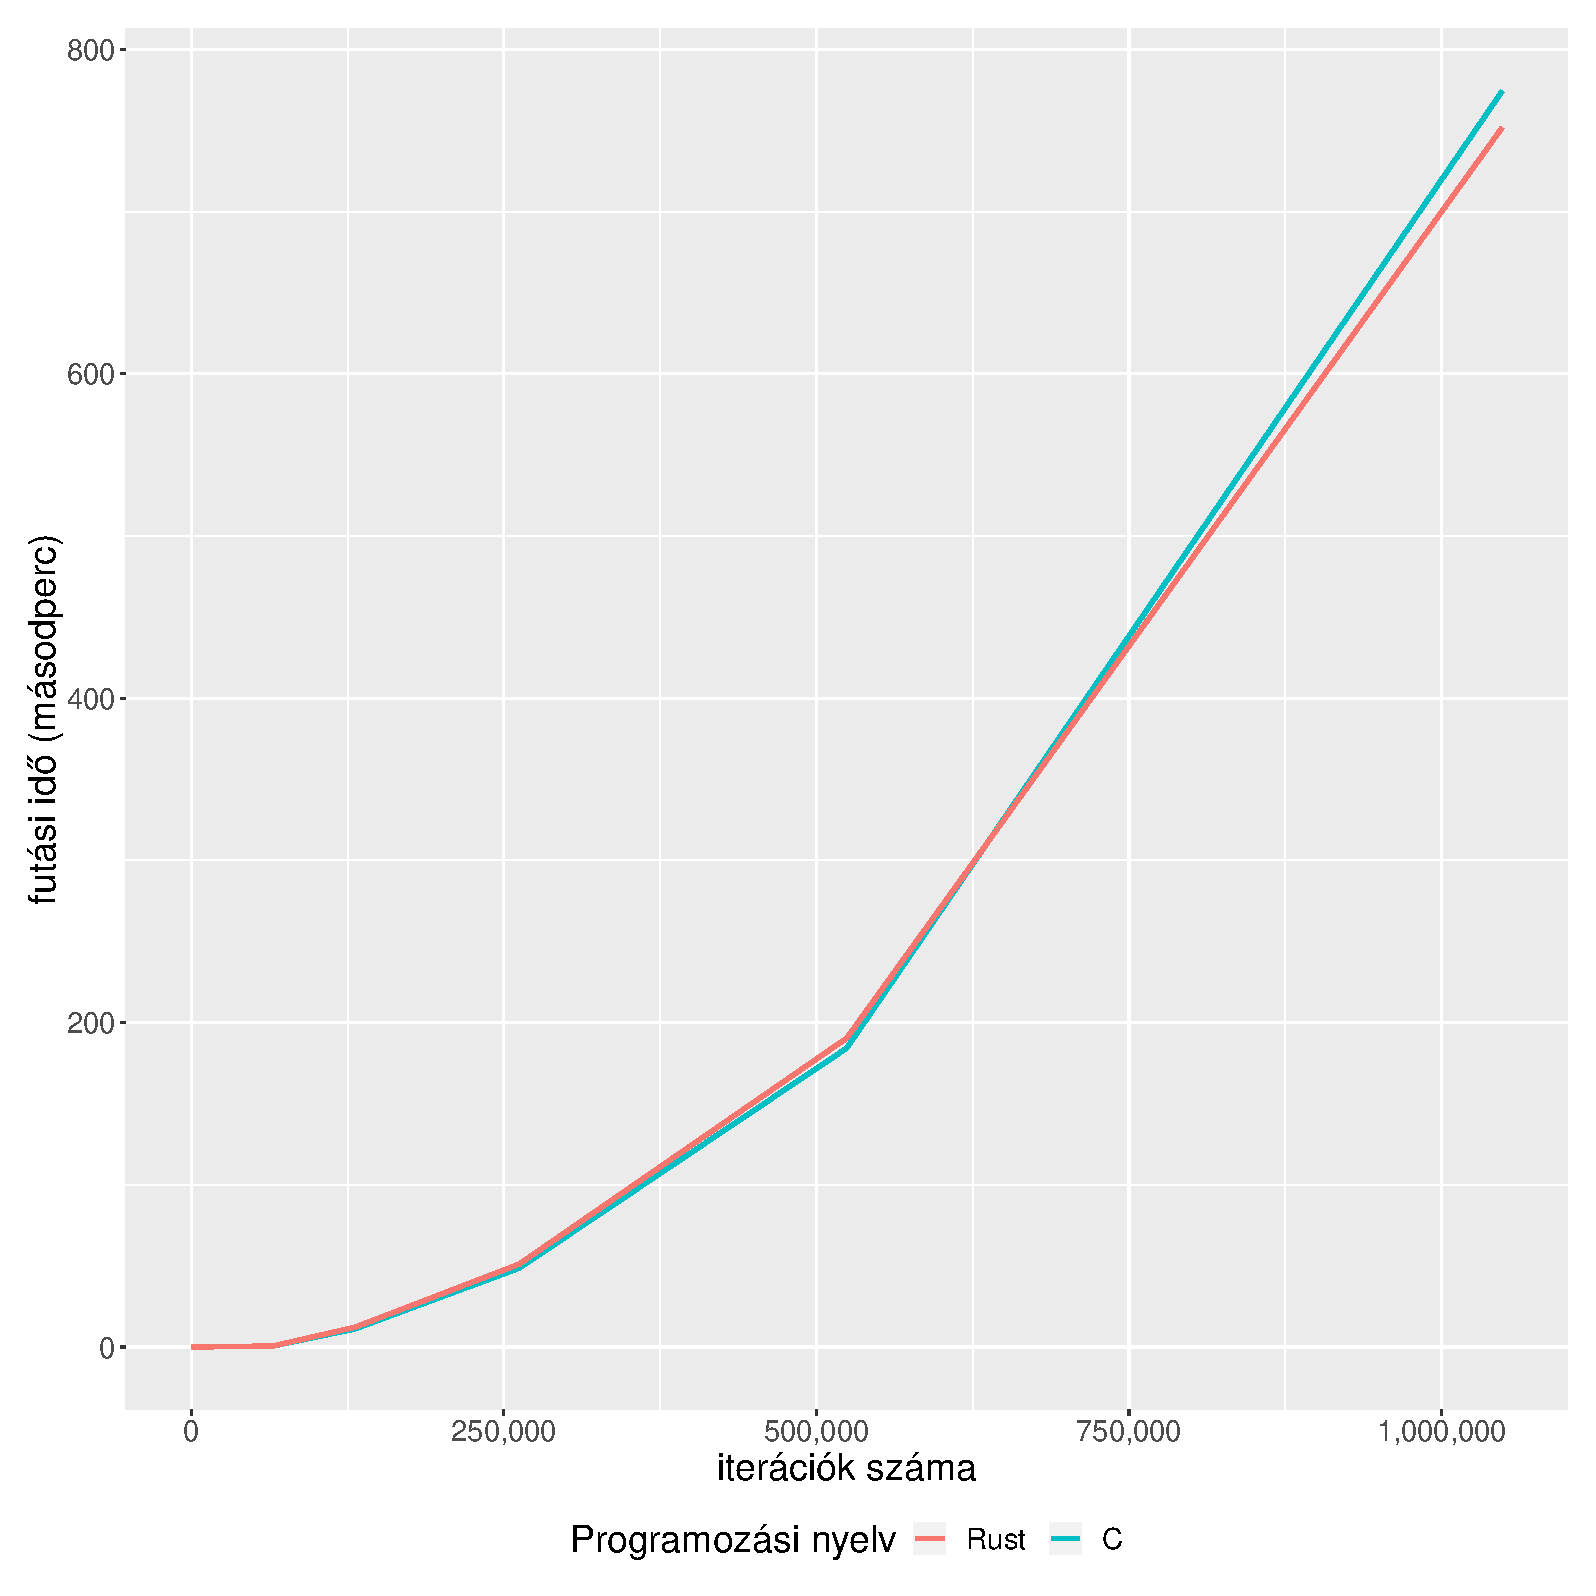
\includegraphics[width=15.5cm]{kepek/trapedozial_rule_run.eps}

\subsection{Iteratív Simpson-módszer}

\subsubsection{Rövid matematikai bevezetés}

A Simpson-módszer a trapézszabályon alapul úgy, hogy a részintervallumok végpontjaihoz súlyokat rendel. Az iteratív Simpson-módszer a Simpson-módszerre alapul, az iteratív trapézszabályhoz hasonlóan finomítja egyre jobban a közelítést minden iterációban.

\subsubsection{C nyelvű referencia-implementáció}
A Simpson-módszer implementációja hasonló az iteratív trapézszabályékhoz, a különbséget a közelítő érték kiszámításához használatos formula jelenti.
\cppstyle{\begin{lstlisting}[language=c++]
float q_simpsons_rule(float a, float b, int j_max) {
    const float EPS = 0.00000001;
    const int J_MIN_ITERATION_COUNT = 5;

    float s = 0.0;
    float st;
    float ost;
    float os;

    os = -0.00000000000000000000000000001;
    ost = os;

    for (int j = 0; j < j_max; j++) {
        st = trapedozial_rule(a, b, j);
        s = (4.0 * st - ost) / 3.0;
        if (j > J_MIN_ITERATION_COUNT) {
            if (abs_float(s - os) < EPS * abs_float(os) || (s == 0.0 && os == 0.0) ) {
                return s;
            }
        }
        os = s;
        ost = st;
    }
    return s;
}
\end{lstlisting}}
\subsubsection{Az algoritmus egy implementációja Rustban}
Az algoritmus Rust nyelvű implementációja, jelentős különbségek ebben az esetben sincsenek.
\begin{lstlisting}[language=Rust]
pub fn q_simpsons_rule(a: f32, b: f32, j_max: i32) -> f32 {
    const EPS: f32 = 0.000000001;
    const J_MIN_ITERATION_COUNT: i32 = 5;

    let mut s: f32 = 0.0;
    let mut st: f32;
    let mut ost: f32;
    let mut os: f32;

    os = -0.00000000000000000000000000001;
    ost = os;

    for j in 0..j_max {
        st = trapedozial_rule(a, b, j);
        s = (4.0 * st - ost) / 3.0;
        if j > J_MIN_ITERATION_COUNT {
            if (s - os).abs() < EPS * os.abs() || (s == 0.0 && os == 0.0) {
                return s;
            }
        }
        os = s;
        ost = st;
    }
    return s;
}
\end{lstlisting}
\subsubsection{Futtatások eredményei}
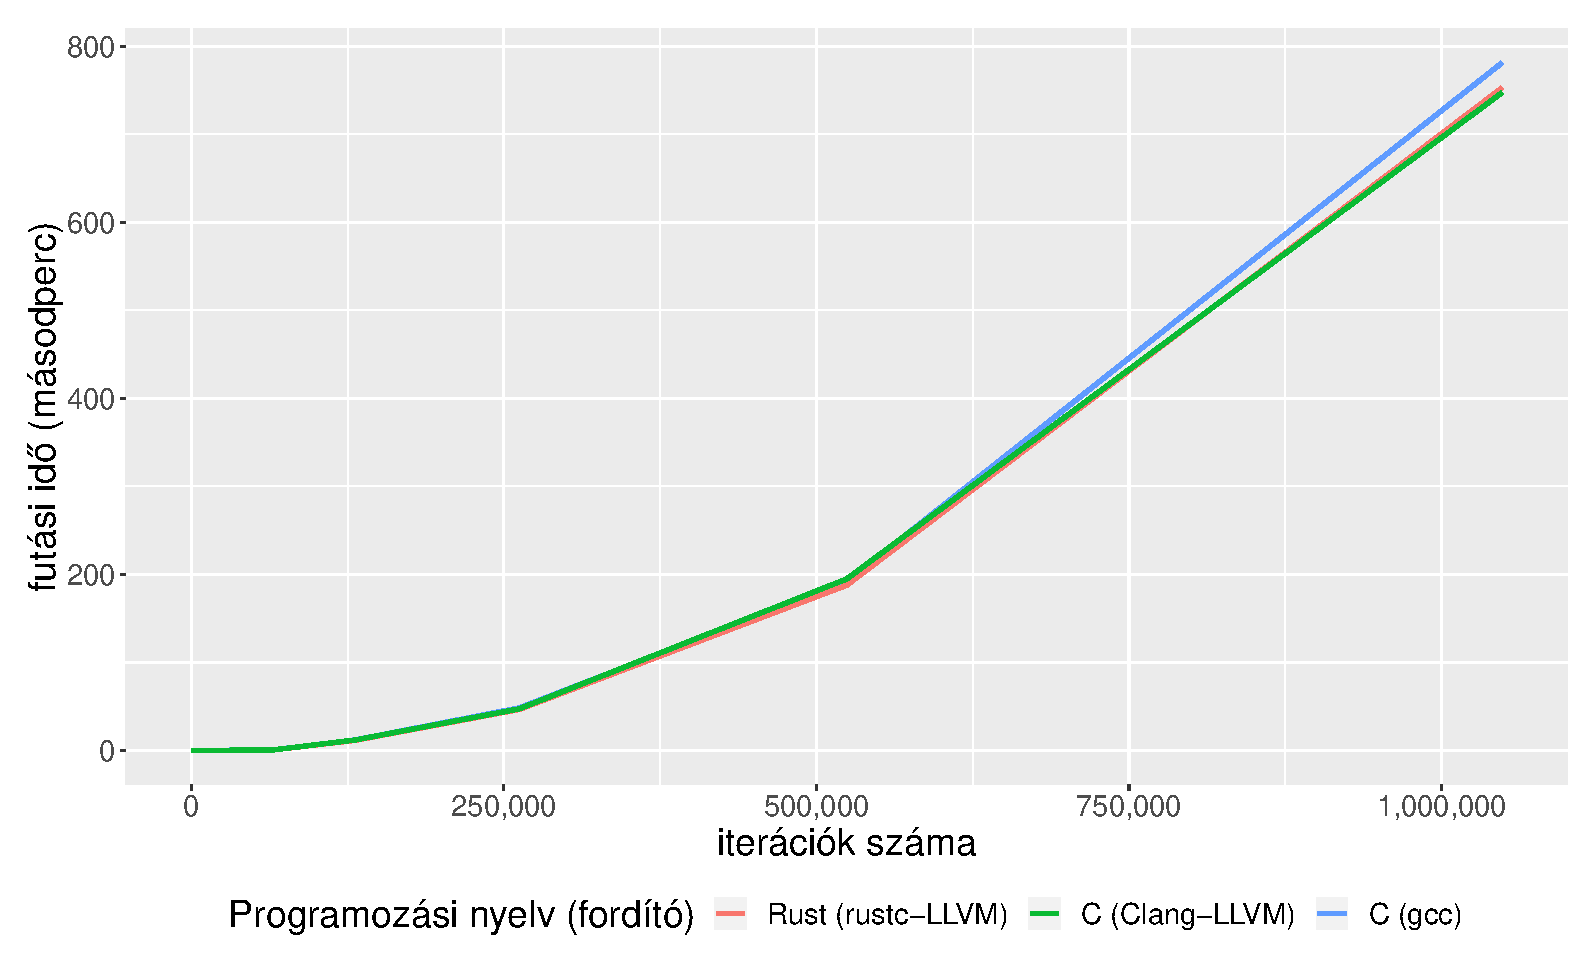
\includegraphics[width=15.5cm]{kepek/simpsons_rule_run.eps}

\section{Rendezés}

\subsection{Kupacrendezés}

\subsubsection{Rövid matematikai bevezetés}

A kupacrendezés két részre osztja az inputot: egy rendezett és egy nem rendezett részre. A gyökérelem (legnagyobb elem) megkeresésével és a rendezett részbe mozgatásával egyre csökkenti a nem rendezett rész méretét. Legrosszabb esetben is \[ \Theta(n log n)\] időkomplexitással rendelkezik.

\subsubsection{C nyelvű referencia-implementáció}

\cppstyle{\begin{lstlisting}[language=c++]
void heapify(Vec *a, unsigned n, unsigned i) {
    unsigned largest = i;
    unsigned l = 2 * i + 1;
    unsigned r = 2 * i + 2;

    if ((r < n) && (a->elements[i] < a->elements[l])) {
        largest = l;
    }

    if ((r < n) && (a->elements[largest] < a->elements[r]) ) {
        largest = r;
    }

    if (largest != i) {
        SWAP(float, a->elements[largest], a->elements[i]);
        heapify(a, n, largest);
    }
}

void heapsort(unsigned n, Vec *a) {
    unsigned i = n;
    while (i > 0) {
        heapify(a, n, i);
        i -= 1;
    }

    i = n - 1;
    while (i > 0) {
        SWAP(float, a->elements[0], a->elements[i]);
        heapify(a, i ,0);
        i -= 1;
    }
}
\end{lstlisting}}
\subsubsection{Az algoritmus egy implementációja Rustban}
Kiemelendő részlet, hogy a Rust nyelvű implementációban a \lstinline{Vec} típus \lstinline{swap} metódusa került felhasználásra a vektor két elemének megcseréléséhez.
\begin{lstlisting}[language=Rust]
fn heapify(a: &mut Vec<f32>, n: usize, i: usize) {
    let mut largest: usize = i;
    let l = 2 * i + 1;
    let r = 2 * i + 2;

    if r < n && a[i] < a[l] {
        largest = l;
    }

    if r < n && a[largest] < a[r] {
        largest = r;
    }

    if largest != i {
        a.swap(largest, i);

        heapify(a, n, largest);
    }
}

pub fn heapsort(n: usize, a: &mut Vec<f32>) {
    let mut i: usize = n;
    while i > 0 {
        heapify(a, n, i);
        i -= 1;
    }

    i = n - 1;
    while i > 0 {
        a.swap(0, i);
        heapify(a, i, 0);
        i -= 1;
    }
}
\end{lstlisting}
\subsubsection{Futtatások eredményei}
Kupac-rendezés futási ideje

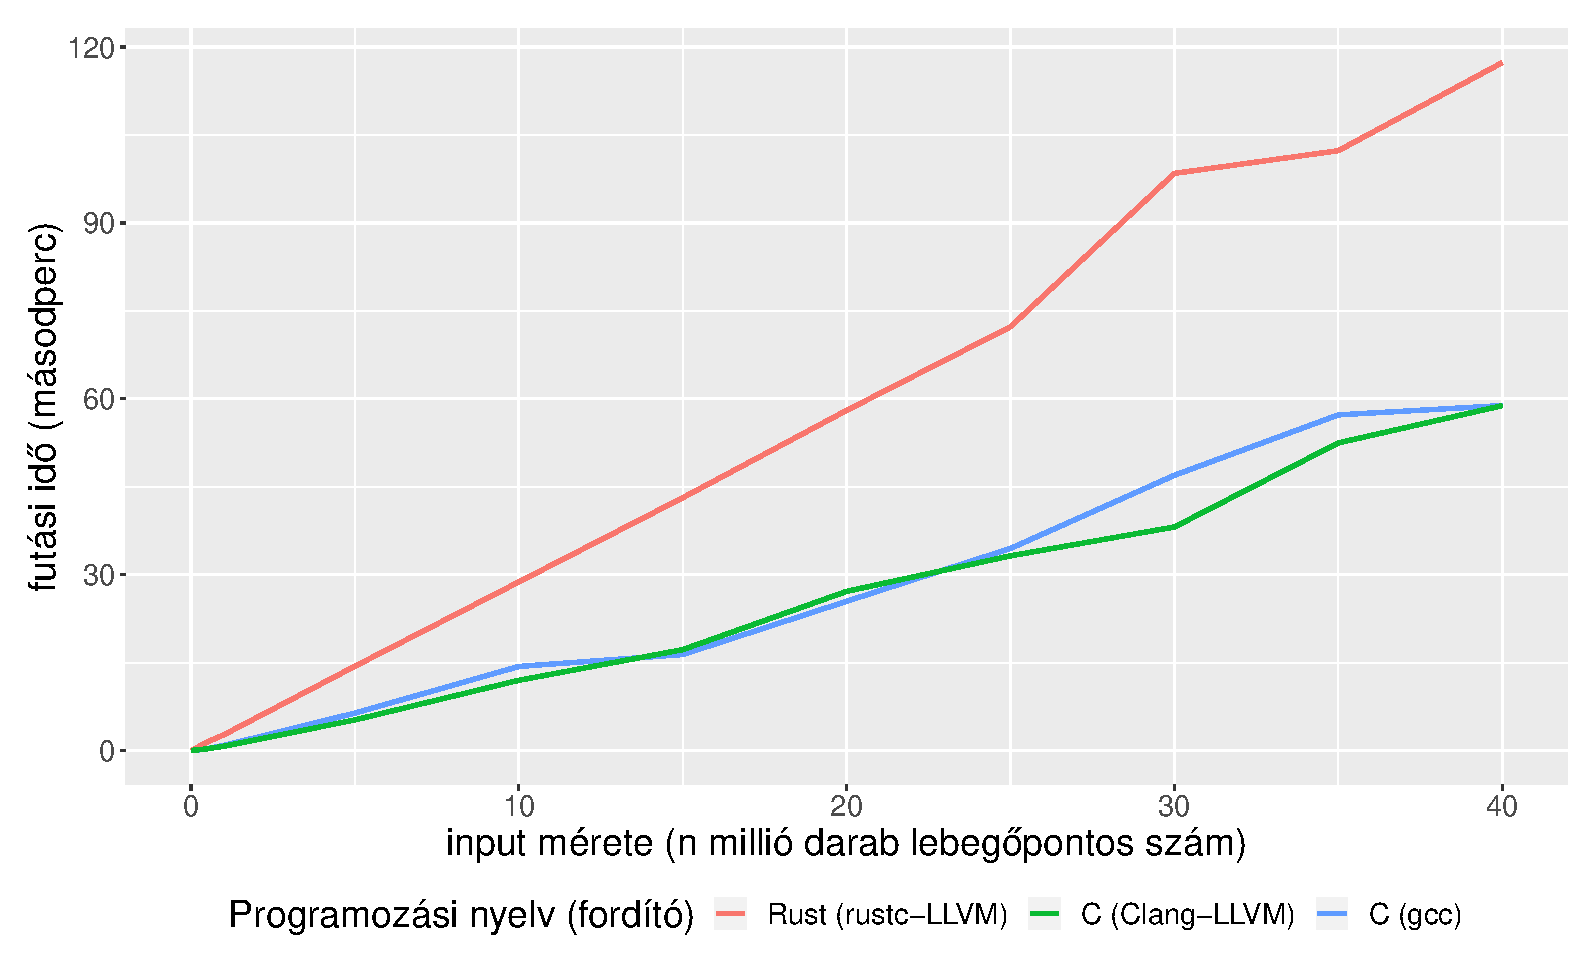
\includegraphics[width=15.5cm]{kepek/heap_sort_run.eps}
Látható, hogy a kupac-rendezés módszerét tekintve a Rust nyelvű implementáció lassabb, mint a C-s megfelelője.

\noindent Kupac-rendezés maximális memóriafoglalása

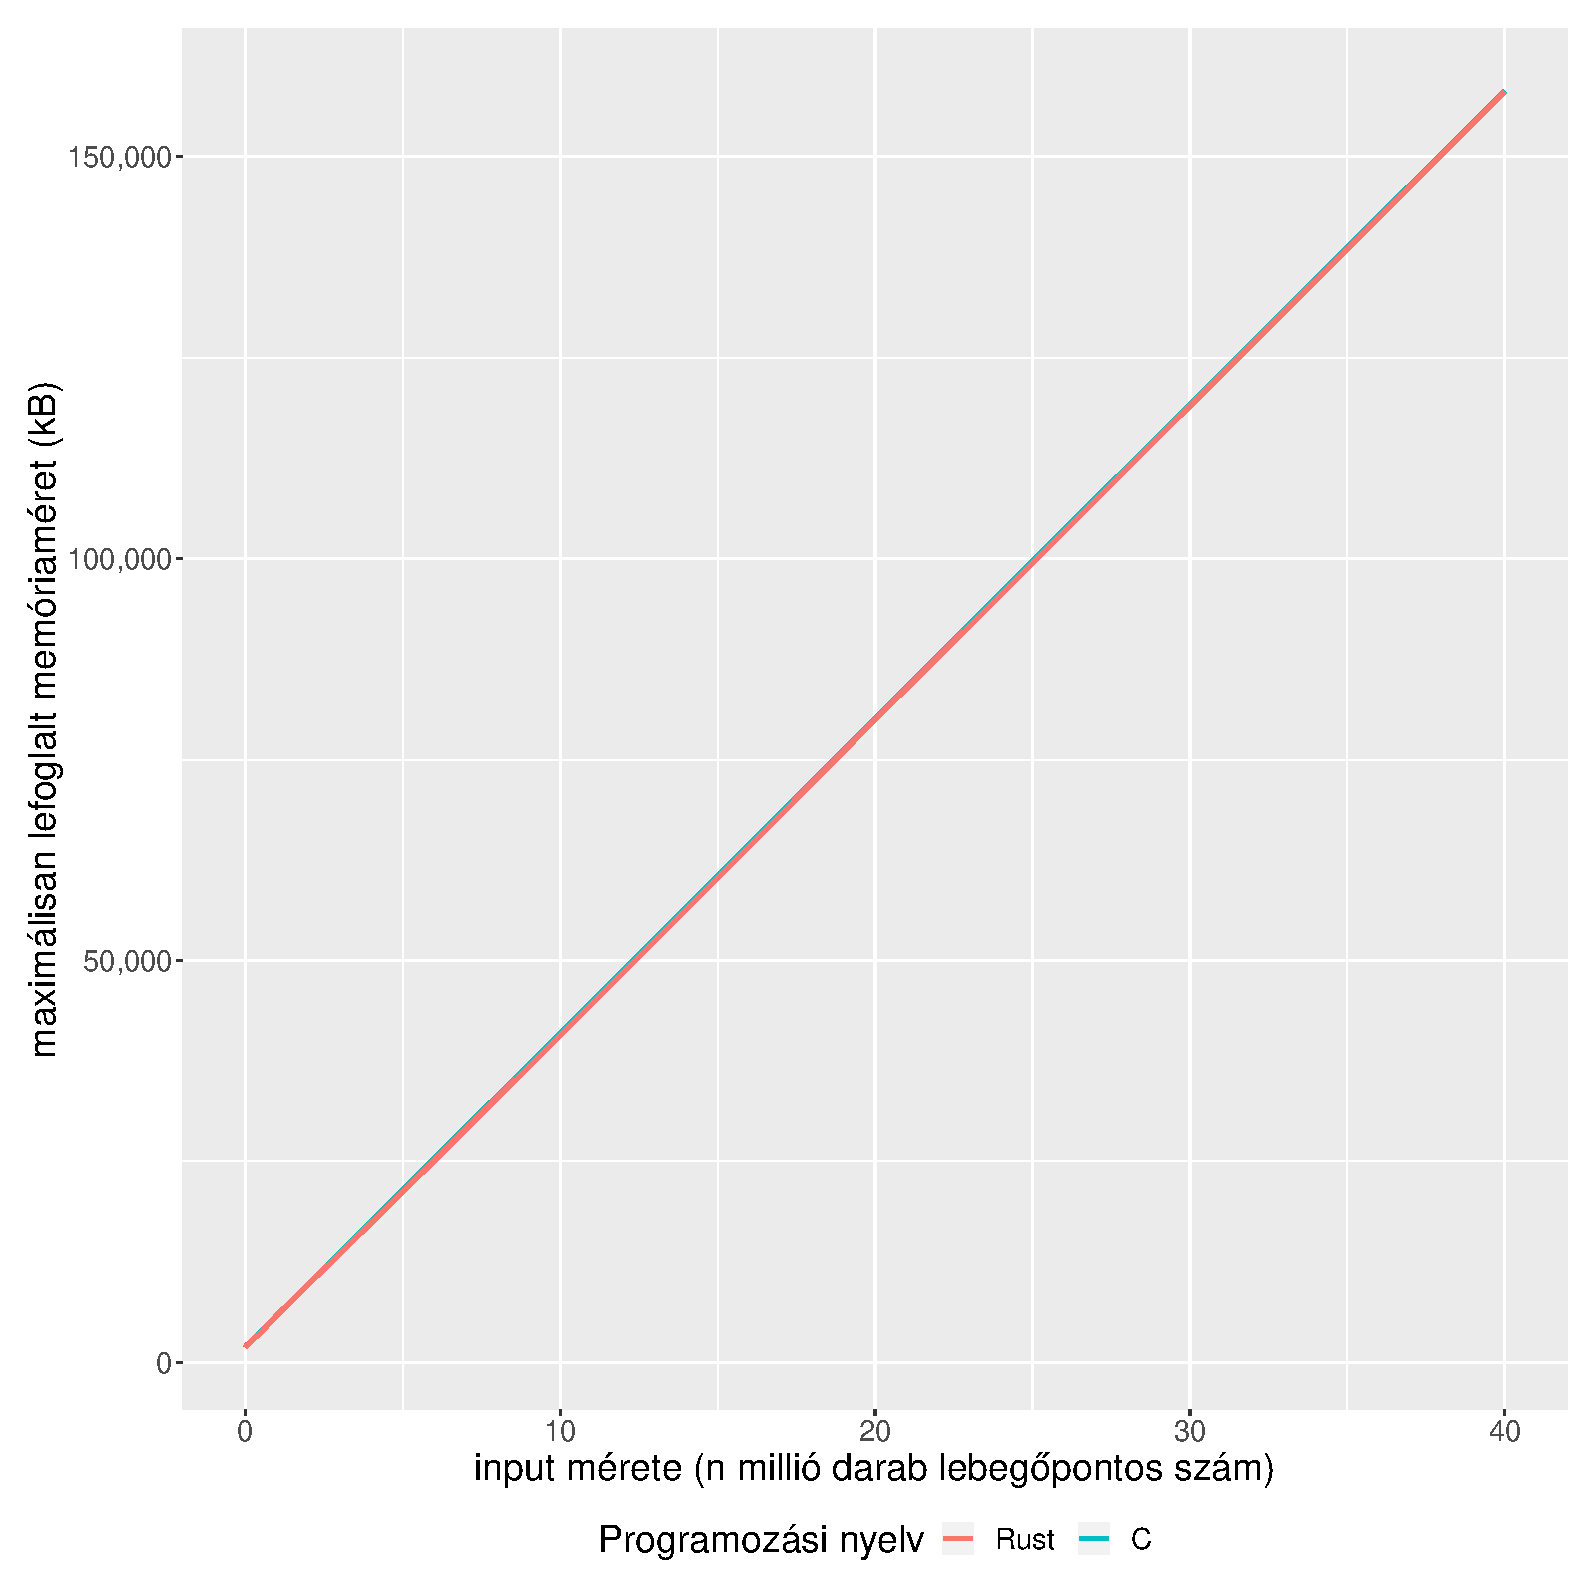
\includegraphics[width=15.5cm]{kepek/heap_sort_memory.eps}
A Rust és C nyelven elkészített implementációk között a maximális memóriafoglalást tekintve nincsenek jelentős eltérések.

\subsection{Shell-rendezés}
\subsubsection{Rövid matematikai bevezetés}
Az egymástól távoli elemek összehasonlításával kezdi a rendezést, majd a szomszédos elemek felé, egyre közelebbi elemeket összehasonlítva, és szükség szerint felcserélve azokat. 

\noindent Elméleti futásidő legjobb és átlagos esetben:
\[\Theta(n log n) \]

\noindent Elméleti futásidő legrosszabb eset:
\[\Theta(n^2)\]

\subsubsection{C nyelvű referencia-implementáció}

\cppstyle{\begin{lstlisting}[language=c++]
void shell_sort(unsigned n, Vec *a) {
    int gap = (n / 2);
    float temp;
    unsigned int i;
    int j;

    while (gap > 0) {
        for (i = gap; i < n; i++) {
            temp = a->elements[i];
            
            j = i;
            while ((j >= gap) && (a->elements[(j-gap)] > temp) ) {
                a->elements[j] = a->elements[(j-gap)];
                j -= gap;
            }
            a->elements[j] = temp;
        }
        gap /= 2;
    }
}
\end{lstlisting}}
\subsubsection{Az algoritmus egy implementációja Rustban}
\begin{lstlisting}[language=Rust]
pub fn shell_sort(n: i32, a: &mut Vec<f32>) {
    let mut gap: i32 = (n / 2) as i32;
    let mut temp: f32;
    let mut j: i32;

    while gap > 0 {
        for i in gap..n {
            temp = a[i as usize];

            j = i;
            while j >= gap && a[(j - gap) as usize] > temp {
                a[j as usize] = a[(j - gap) as usize];
                j -= gap;
            }
            a[j as usize] = temp;
        }
        gap /= 2;
    }
}
\end{lstlisting}
\subsubsection{Futtatások eredményei}
Shell-rendezés futási ideje

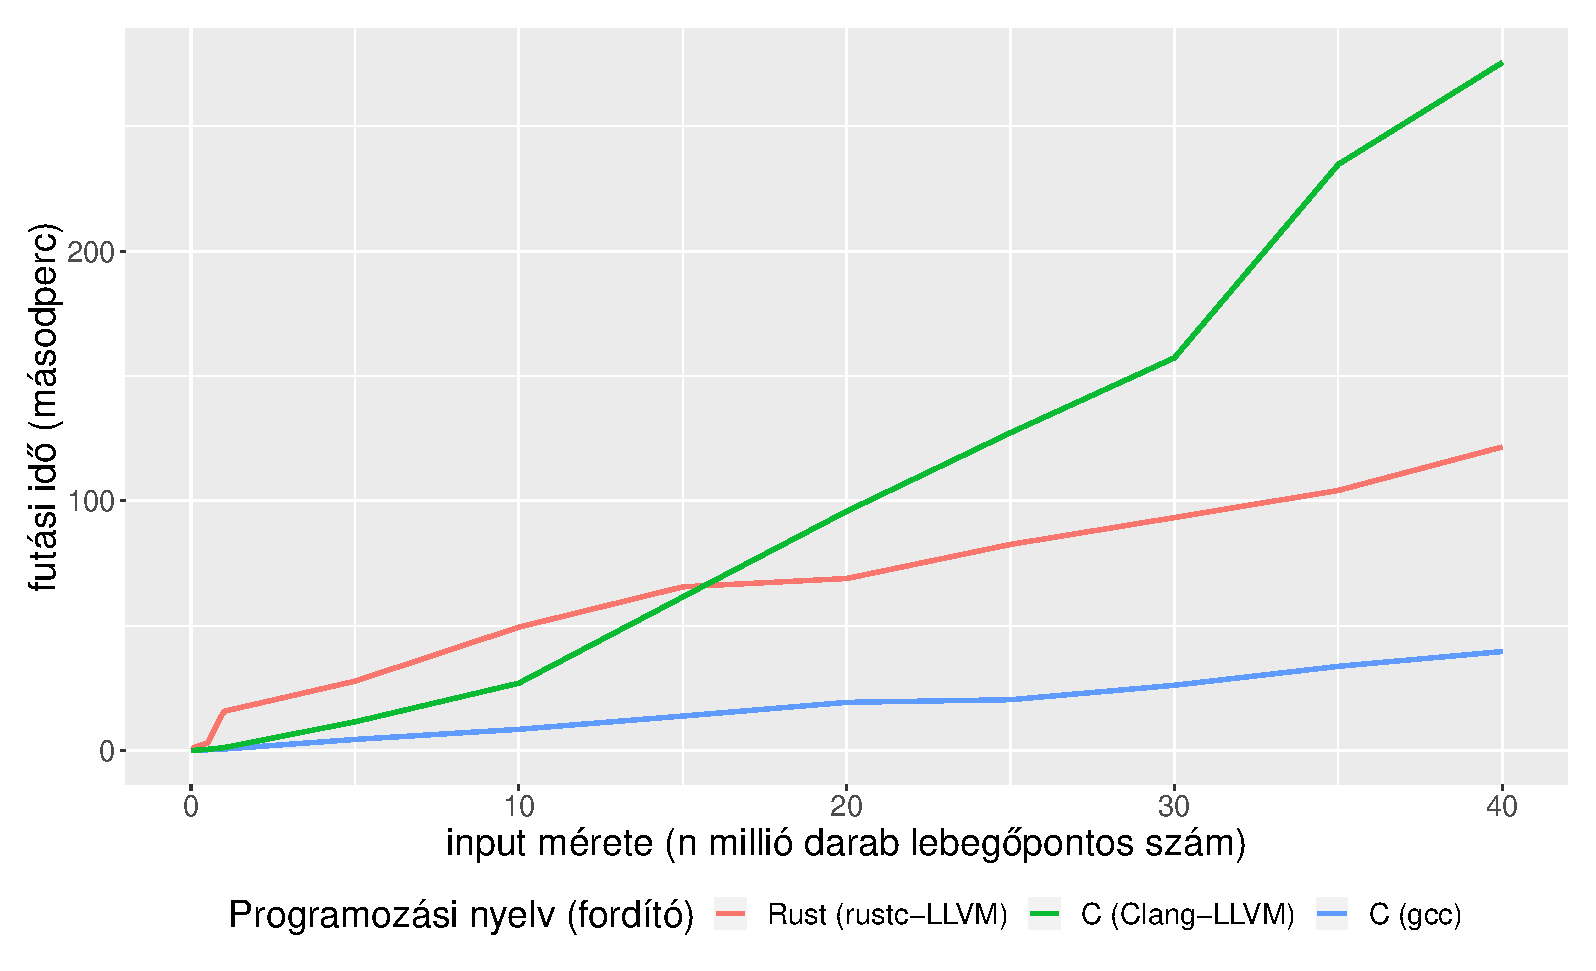
\includegraphics[width=15.5cm]{kepek/shells_sort_run.eps}
Látható, hogy a Shell-rendezés módszerét tekintve a Rust nyelvű implementáció lassabb, mint a C-s megfelelője.

\noindent Shell-rendezés maximális memóriafoglalása

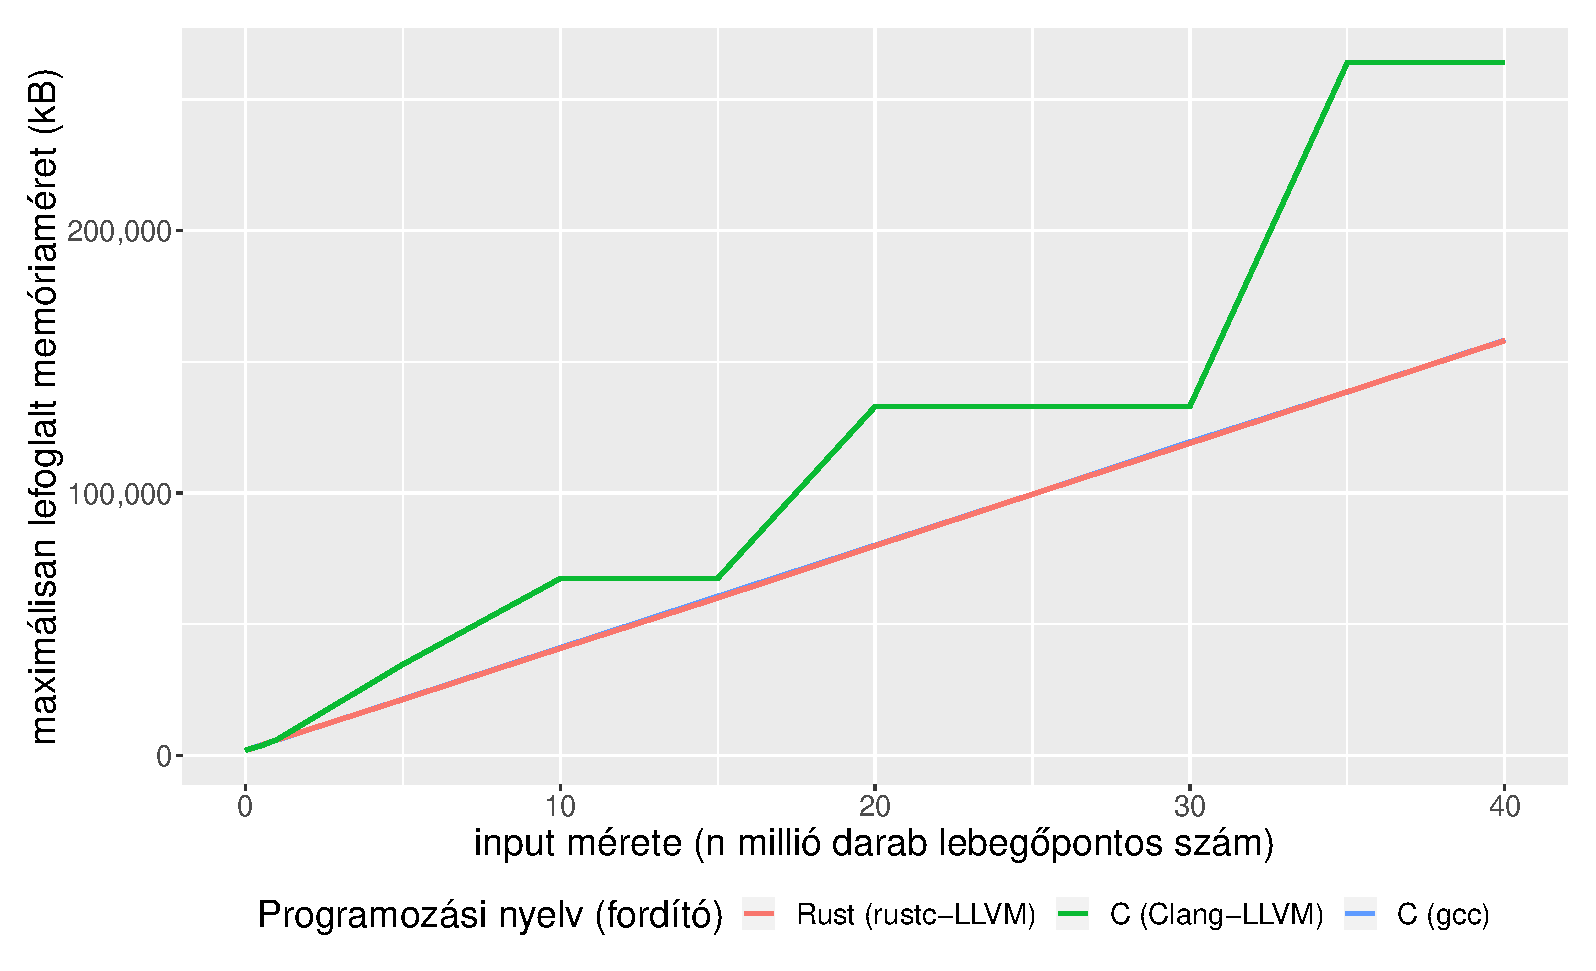
\includegraphics[width=15.5cm]{kepek/shells_sort_memory.eps}
A Rust és C nyelven elkészített implementációk között a maximális memóriafoglalást tekintve nincsenek jelentős eltérések.

\subsection{Gyorsrendezés (Quicksort)}
\subsubsection{Rövid matematikai bevezetés}
A gyorsrendezés egy rekurzív algoritmus, amely az „oszd meg és uralkodj” elve alapján működik. Az input elemeket két részre osztja az alapján, hogy egy kiválasztott (pivot) elemtől kisebbek, vagy nagyobbak. Az így létrejött két részre meghívásra kerül a gyorsrendezés, egészen addig, amíg egy elemű részek nem jönnek létre. Egyetlen elem mindig rendezett. Az implementációban a Robert Sedgewick ajánlásának megfelelően kerül kiválasztásra a pivot elem, így elkerülhető a legrosszabb eset, a már rendezett elemek listája.

Elméleti futásidő legjobb és átlagos esetben:
\[\Theta(n log n) \]

Elméleti futásidő legrosszabb eset:
\[\Theta(n^2)\]
 
\subsubsection{C nyelvű referencia-implementáció}
\cppstyle{\begin{lstlisting}[language=c++]
int partition(int low, int high, Vec *arr) {
    float pivot;

    int mid = (low + high) / 2;
    if (arr->elements[mid] < arr->elements[low]) {
        SWAP(float, arr->elements[low], arr->elements[high]);
    }

    if (arr->elements[high] < arr->elements[low]) {
        SWAP(float, arr->elements[low], arr->elements[high]);
    }

    if (arr->elements[mid] < arr->elements[high]) {
        SWAP(float, arr->elements[mid], arr->elements[high]);
    }

    pivot = arr->elements[high];

    int i;
    int j;

    i = low - 1;
	  j = high + 1;

    while (1) {
        while (1) {
            i += 1;
            if (arr->elements[i] >= pivot) {
                break;
            }
        }

        while (1) {
            j -= 1;
            if (arr->elements[j] <= pivot) {
                break;
            }
        }

        if (i >= j) {
            return j;
        }

        SWAP(float, arr->elements[i], arr->elements[j]);
    }
}

void quicksort(int low, int high, Vec *arr) {
    if (low < high) {
        int p = partition(low, high, arr);
        quicksort(low, p, arr);
        quicksort(p+1, high, arr);
    } else {
        return;
    }
}
\end{lstlisting}}
\subsubsection{Az algoritmus egy implementációja Rustban}
\begin{lstlisting}[language=Rust]
pub fn quicksort(low: i32, high: i32, arr: &mut Vec<f32>) {
    if low < high {
        let p: i32 = partition(low, high, arr);
        quicksort(low, p, arr);
        quicksort(p + 1, high, arr);
    } else {
        return;
    }
}

fn partition(low: i32, high: i32, arr: &mut Vec<f32>) -> i32 {
    let pivot: f32;

    let mid: i32 = (low + high) / 2;
    if arr[mid as usize] < arr[low as usize] {
        arr.swap(low as usize, high as usize);
    }
    if arr[high as usize] < arr[low as usize] {
        arr.swap(low as usize, high as usize);
    }
    if arr[mid as usize] < arr[high as usize] {
        arr.swap(mid as usize, high as usize);
    }
    pivot = arr[high as usize];

    let mut i: i32;
    let mut j: i32;

    i = low - 1;
    j = high + 1;

    loop {
        loop {
            i += 1;
            if arr[i as usize] >= pivot {
                break;
            }
        }

        loop {
            j -= 1;
            if arr[j as usize] <= pivot {
                break;
            }
        }

        if i >= j {
            return j as i32;
        }

        arr.swap(i as usize, j as usize);
    }
}

\end{lstlisting}
\subsubsection{Futtatások eredményei}
Gyorsrendezés futási ideje

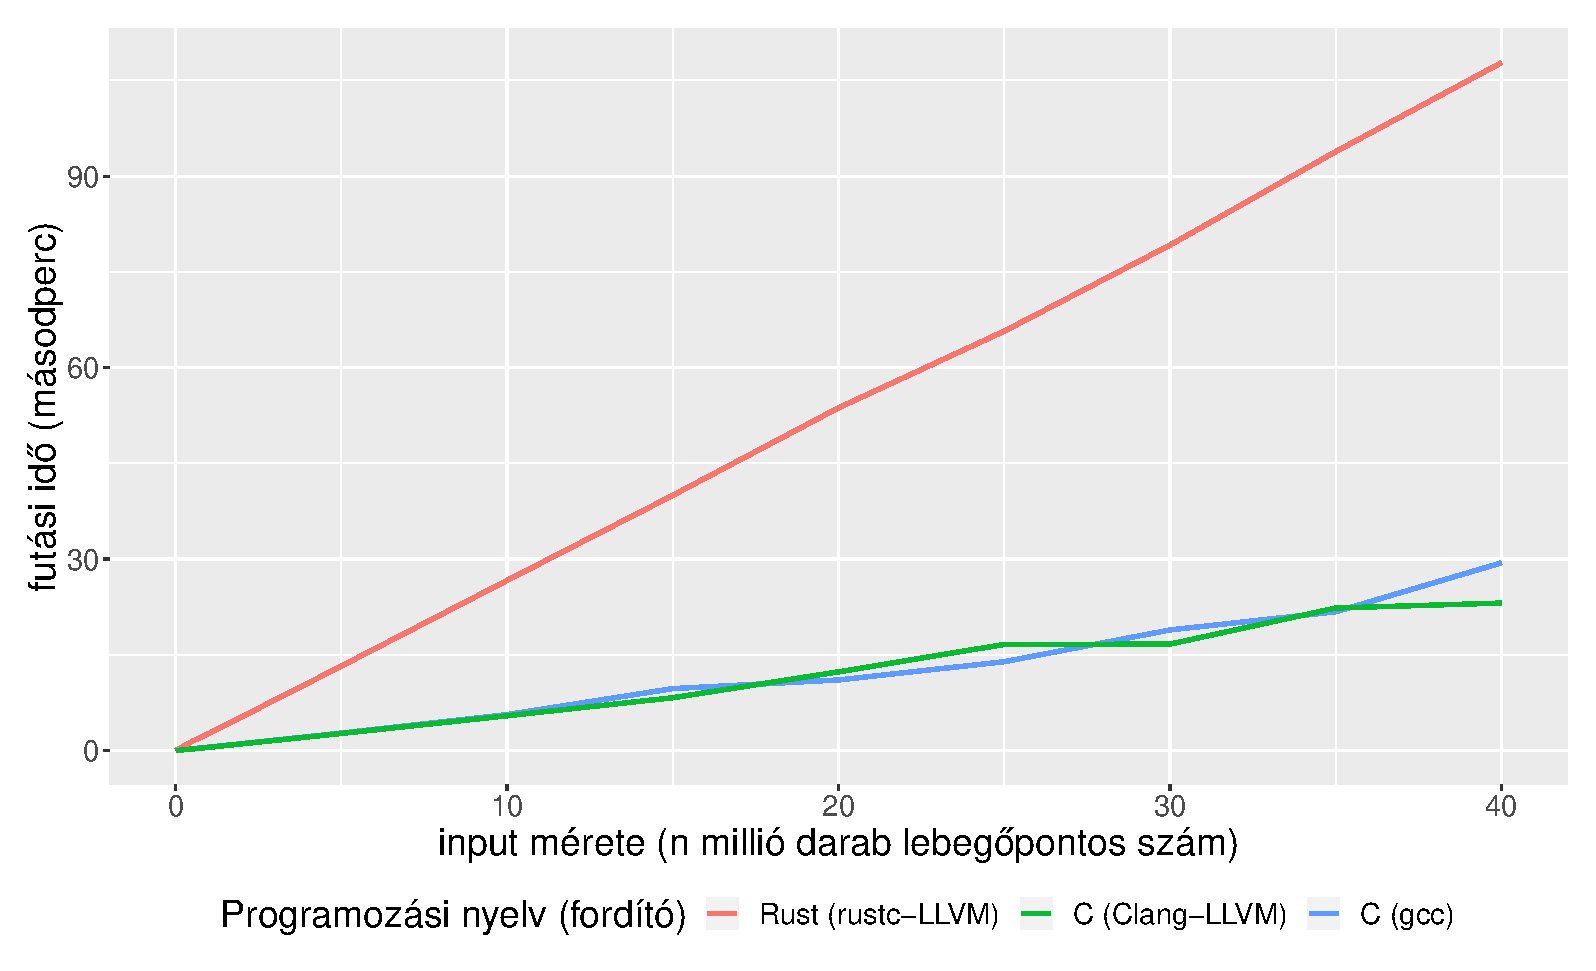
\includegraphics[width=15.5cm]{kepek/quicksort_run.eps}
Látható, hogy a gyorsrendezés módszerét tekintve a Rust nyelvű implementáció lassabb, mint a C-s megfelelője.

\noindent Gyorsrendezés maximális memóriafoglalása

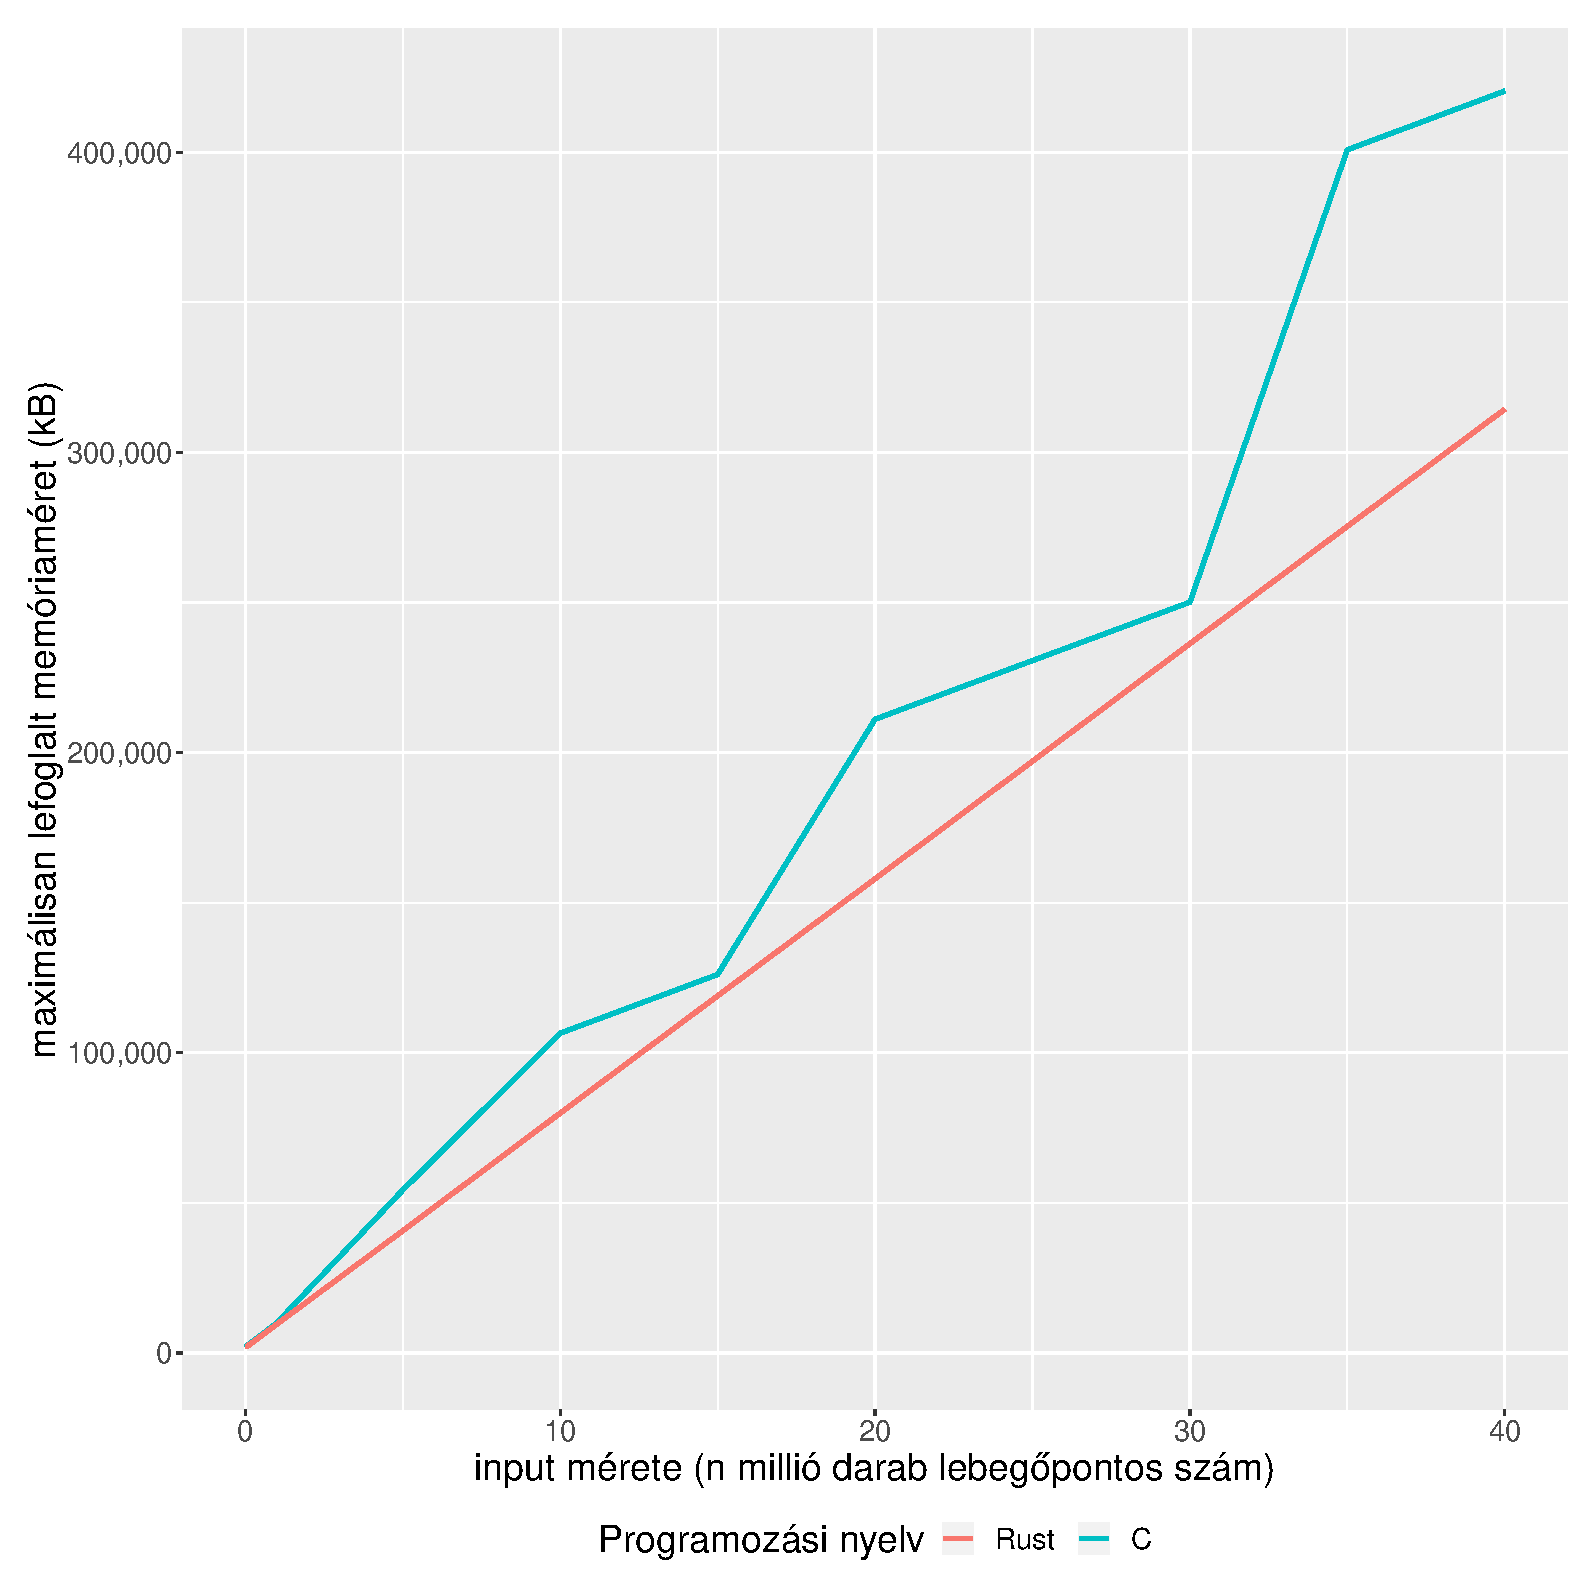
\includegraphics[width=15.5cm]{kepek/quicksort_memory.eps}
A Rust és C nyelven elkészített implementációk között a maximális memóriafoglalást tekintve nincsenek jelentős eltérések.

\section{Interpoláció}

\subsection{Lineáris interpoláció}
\subsubsection{Rövid matematikai bevezetés}
A lineáris interpoláció két ismert pont közötti összefüggést egyenes arányossággal közelíti. Az ismert pontok által meghatározott egyenesen lévő pontnak így elég az egyik koordinátáját ismerni a másik koordinátájának kiszámításához.
\[ y_n = \frac{x_n - x_1}{x_2 - x_1} * (y_2 - y_1) + y_1 \]
Ahol $x_1 \neq x_2$.
\subsubsection{C nyelvű referencia-implementáció}
A lineáris interpoláció implementációja egyszerű. Ha a paraméterként kapott két pont \lstinline{x} értékei megegyeznek, akkor az első pont \lstinline{y} értékével tér vissza.
\cppstyle{\begin{lstlisting}[language=c++]
float linear_interpolation(float x1, float y1, float x0, float y0, float x) {
    float delta;
    delta = x1 - x0;
    float y;

    if (delta == 0.0) {
        y = y0;
    } else {
        y = y0 + ( (x - x0) / delta) * y1;
    }

    return y;
}
\end{lstlisting}}
\subsubsection{Az algoritmus egy implementációja Rustban}
A Rust nyelvű implementáció nem mutat az esetleges szintaktikai különbözőségeken felül más eltérést a C nyelvűtől.
\begin{lstlisting}[language=Rust]
fn linear_interpolation(x1: f32, y1: f32, x0: f32, y0: f32, x: f32) -> f32 {
    let delta: f32;
    delta = x1 - x0;
    let y;

    if delta == 0.0 {
        y = y0;
    } else {
        y = y0 + ((x - x0) / delta) * y1;
    }

    return y;
}
\end{lstlisting}
\subsubsection{Futtatások eredményei}
Lineáris interpoláció futási ideje

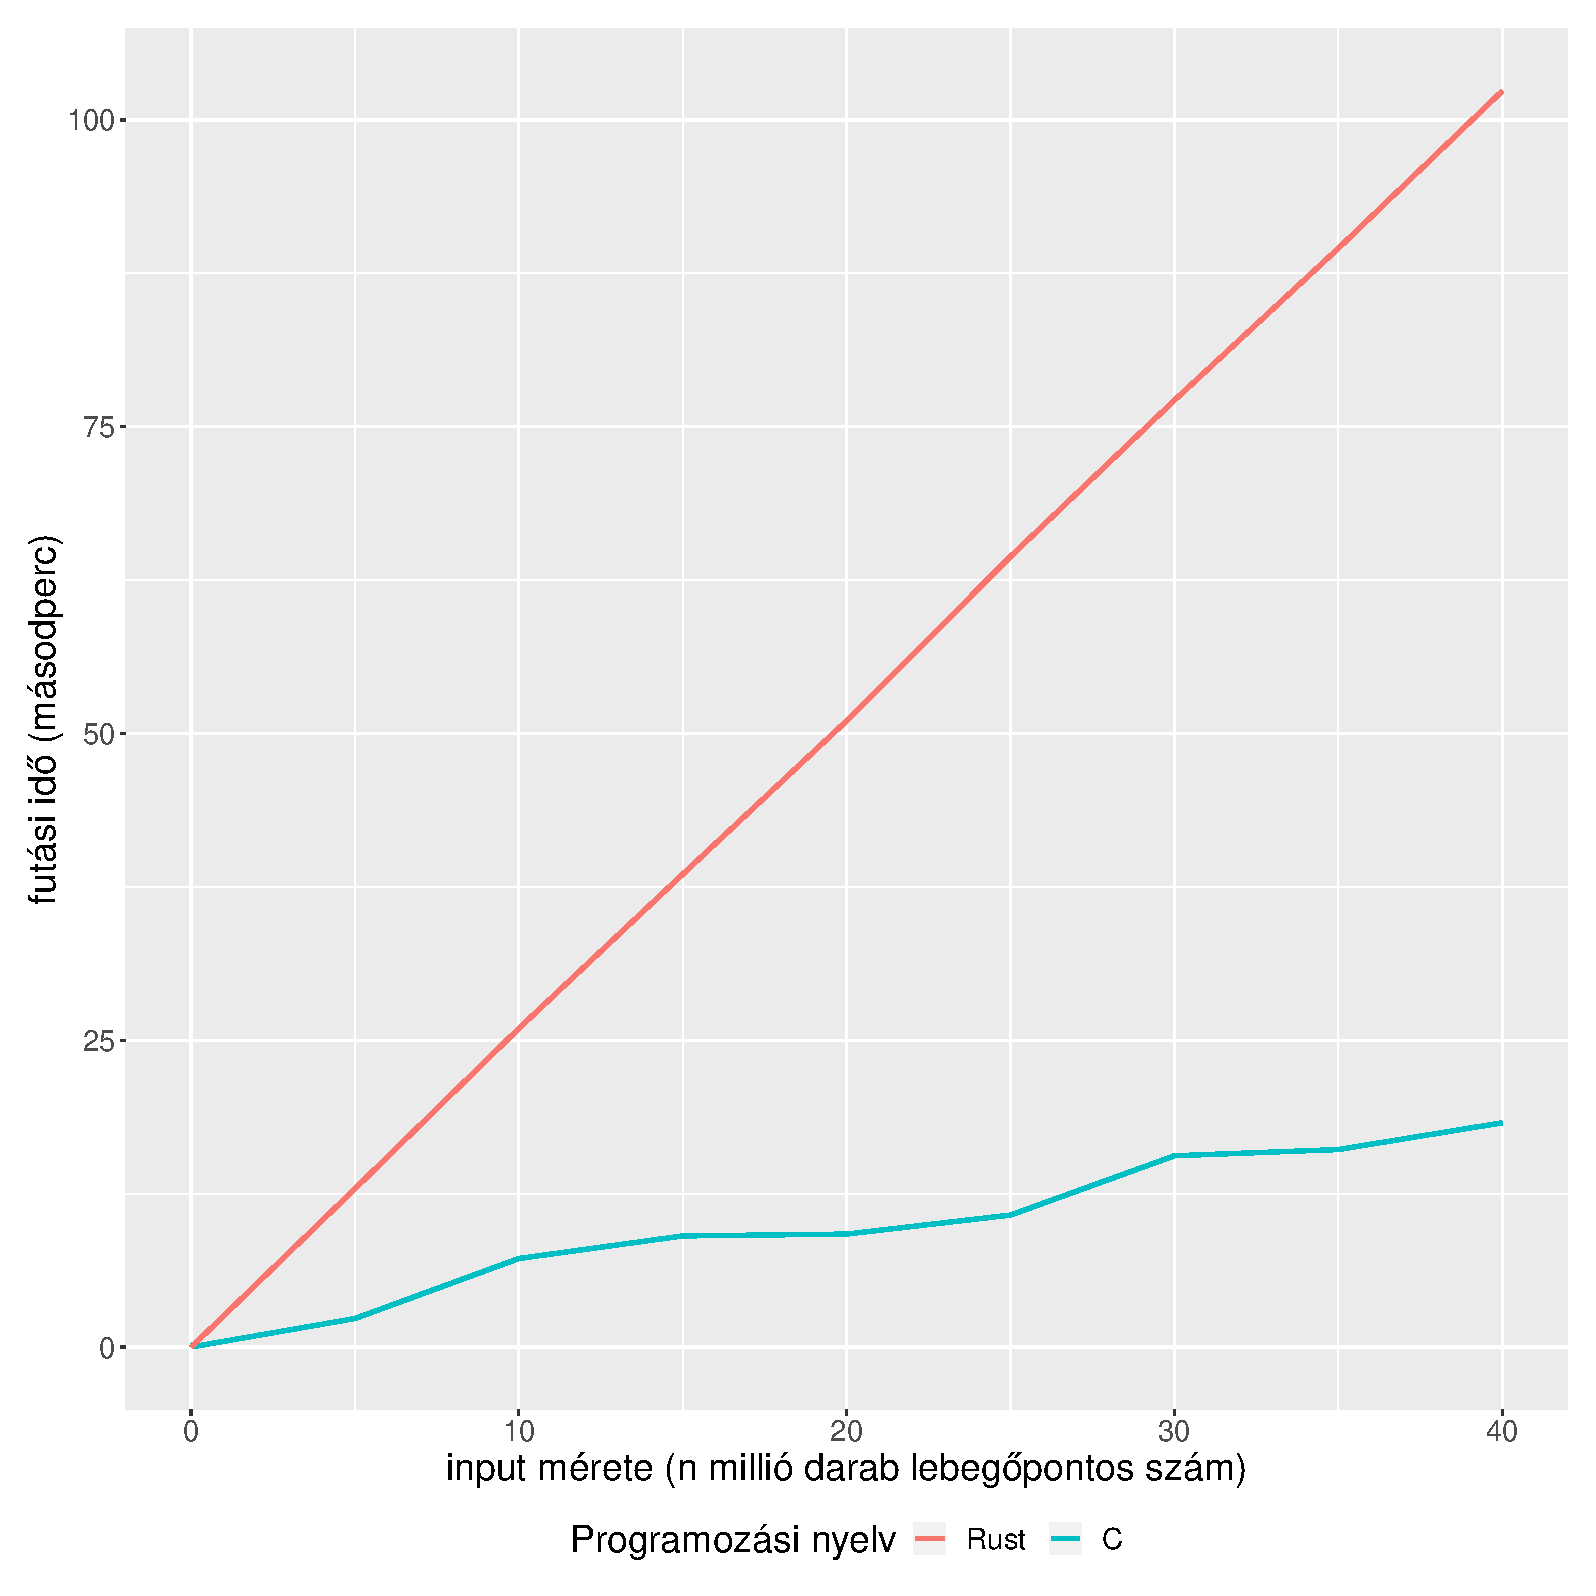
\includegraphics[width=15.5cm]{kepek/linear_interpolation_run.eps}
Látható, hogy a lineáris interpoláció módszerét tekintve a Rust nyelvű implementáció lassabb, mint a C-s megfelelője.


\noindent Lineáris interpoláció maximális memóriafoglalása

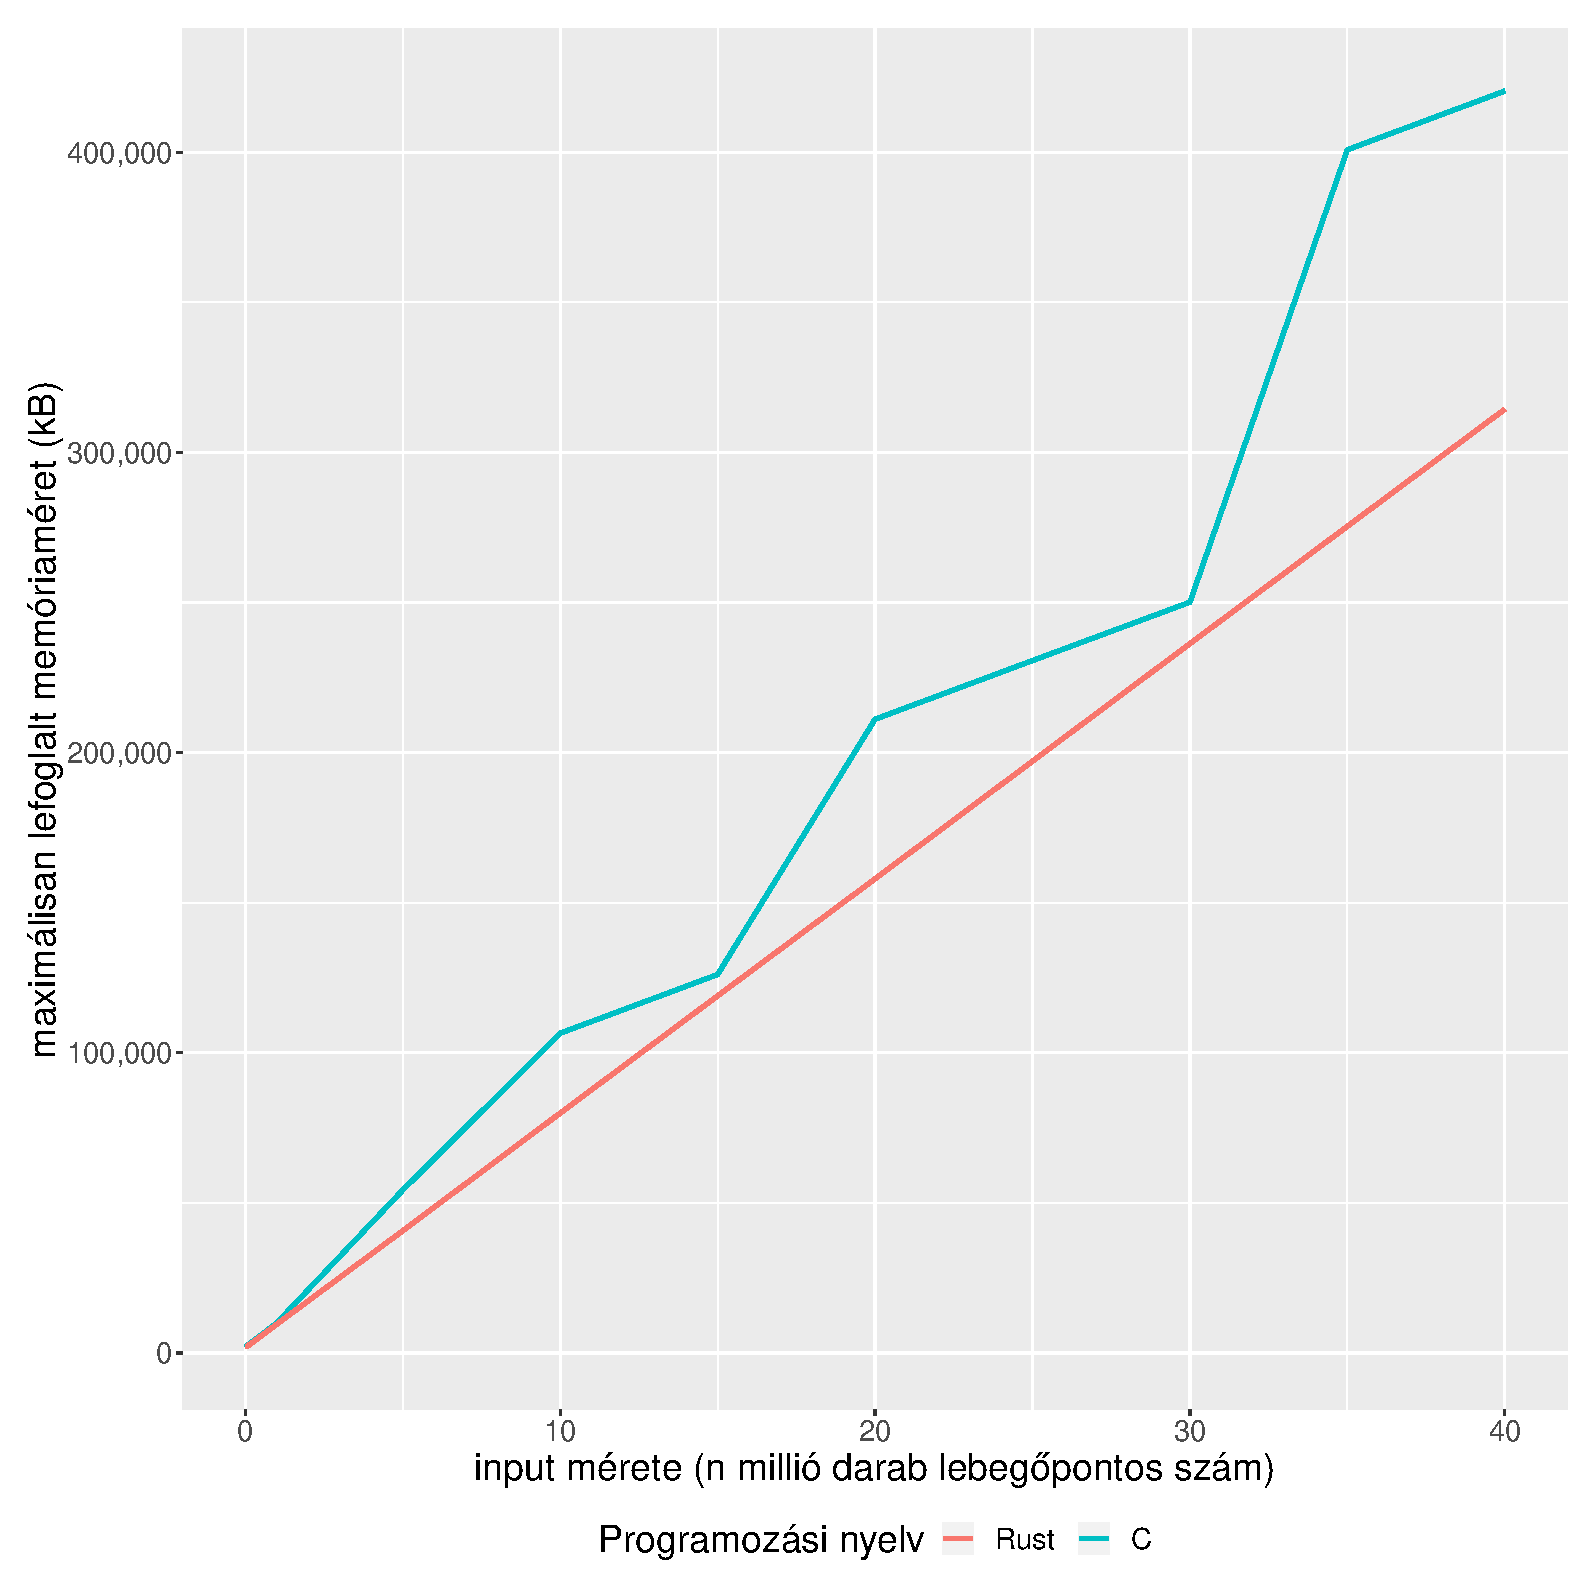
\includegraphics[width=15.5cm]{kepek/linear_interpolation_memory.eps}
A Rust és C nyelven elkészített implementációk között a maximális memóriafoglalást tekintve nincsenek jelentős eltérések.
